\documentclass[12pt, a4paper]{article}

% --- Packages ---
\usepackage[utf8]{inputenc}
\usepackage[T1]{fontenc}
\usepackage[french]{babel}
\usepackage{geometry}
\usepackage{graphicx}
\usepackage{booktabs}
\usepackage{array}
\usepackage{longtable}
\usepackage{multirow}
\usepackage{xcolor}
\usepackage{hyperref}
\usepackage{fancyhdr}
\usepackage{titlesec}
\usepackage{enumitem}
\usepackage{float}
\usepackage{caption}
\usepackage{subcaption}
\usepackage{amsmath}
\usepackage{setspace}
\usepackage{microtype}
\usepackage{parskip}

% --- Mise en page ---
\geometry{
    top=2.5cm,
    bottom=2.5cm,
    left=2.8cm,
    right=2.8cm
}

% --- Couleurs ---
\definecolor{togored}{RGB}{255, 0, 0}
\definecolor{togoyellow}{RGB}{255, 215, 0}
\definecolor{togodark}{RGB}{34, 34, 34}
\definecolor{togogreen}{RGB}{0, 128, 0}
\definecolor{accentblue}{RGB}{33, 150, 243}
\definecolor{lightgray}{RGB}{245, 245, 245}
\definecolor{sectioncolor}{RGB}{27, 94, 32}

% --- Typographie sections ---
\titleformat{\section}
  {\large\bfseries\color{sectioncolor}}
  {\thesection.}{0.8em}{}[\vspace{0.1em}\hrule\vspace{0.3em}]

\titleformat{\subsection}
  {\normalsize\bfseries\color{togodark}}
  {\thesubsection.}{0.6em}{}

\titleformat{\subsubsection}
  {\normalsize\itshape\color{togodark}}
  {\thesubsubsection.}{0.5em}{}

% --- En-tête et pied de page ---
\pagestyle{fancy}
\fancyhf{}
\fancyhead[L]{\small\textit{Tissu Agricole du Togo - Analyse Géospatiale}}
\fancyhead[R]{\small\textit{Data Challenge Agriculture \#1}}
\fancyfoot[C]{\thepage}
\renewcommand{\headrulewidth}{0.4pt}

% --- Hyperlinks ---
\hypersetup{
    colorlinks=true,
    linkcolor=sectioncolor,
    urlcolor=accentblue,
    citecolor=togodark,
    pdftitle={Analyse du Tissu Agricole au Togo},
    pdfauthor={Data Challenge Agriculture \#1},
}

% --- Espacement ---
\setstretch{1.15}

% ============================================================
\begin{document}
% ============================================================

% --- Page de titre ---
\begin{titlepage}
    \centering
    \vspace*{1.5cm}

    % Logo
    
\includegraphics[width=4cm]{images/LOGO.jpg}

    \vspace{1.2cm}

    {\Large\bfseries\color{sectioncolor}
        République Togolaise\\[0.3em]
        Ministère de l'Agriculture, de l'Élevage et du Développement Rural
    }

    \vspace{1.5cm}
    \hrule height 2pt
    \vspace{0.6cm}

    {\Huge\bfseries\color{togodark}
        Analyse Géospatiale du\\[0.4em]
        Tissu Agricole au Togo
    }

    \vspace{0.4cm}
    \hrule height 2pt
    \vspace{1.2cm}

    {\large\itshape
        Tableau de bord interactif - Rapport d'analyse\\[0.5em]
        \textbf{Data Challenge Agriculture \#1 -- Togo AI Lab}
    }

    \vspace{2cm}

    \begin{tabular}{ll}
        \textbf{Auteur :} & OURO-TAGBA Bastou \\[0.3em]
        \textbf{Sources de données :} & geodata.gouv.tg · opendata.gouv.tg \\[0.3em]
        \textbf{Période des données :} & 2024 \\[0.3em]
        \textbf{Date de soumission :} & 22 juin 2026 \\[0.3em]
        \textbf{Outil :} & Dashboard Streamlit interactif \\
    \end{tabular}

    \vfill

    {\small\color{gray}
        Données libres -- geodata.gouv.tg \& opendata.gouv.tg\\
        Traitement et visualisation : Python, Streamlit, Folium, Plotly
    }
\end{titlepage}

% --- Table des matières ---
\newpage
\tableofcontents
\newpage

% ============================================================
\section{Introduction}
% ============================================================

Le secteur agricole constitue l'un des piliers fondamentaux de l'économie togolaise, employant une large part
de la population active et contribuant significativement au Produit Intérieur Brut du pays. Comprendre la
répartition géographique des acteurs et infrastructures agricoles est un préalable essentiel à toute politique
de développement rural efficace.

Dans le cadre du \textbf{Data Challenge Agriculture \#1} organisé par le Togo AI Lab, ce rapport présente
les résultats d'une analyse géospatiale complète du tissu agricole togolais, s'appuyant sur les données
ouvertes disponibles sur les plateformes \texttt{geodata.gouv.tg} et \texttt{opendata.gouv.tg}.

\subsection{Objectifs de l'analyse}

L'objectif principal de ce travail est de concevoir un tableau de bord interactif permettant de :

\begin{itemize}[leftmargin=1.5em]
    \item \textbf{Cartographier} l'ensemble du tissu agricole togolais (exploitations, coopératives, marchés,
          pépinières, zones aménagées) ;
    \item \textbf{Analyser les densités} et distributions géographiques par région, préfecture et commune ;
    \item \textbf{Évaluer la couverture} des Zones d'Aménagement Agricole Planifiées (ZAAPs) ;
    \item \textbf{Mesurer l'accessibilité} aux services agricoles (marchés, coopératives, pépinières) ;
    \item \textbf{Identifier les disparités territoriales} pour orienter les investissements publics.
\end{itemize}

\subsection{Périmètre géographique}

L'analyse couvre l'ensemble du territoire togolais, structuré en \textbf{5 régions administratives} :
Maritime, Plateaux, Centrale, Kara et Savanes. Chaque région est découpée en préfectures, communes,
cantons et localités, permettant une granularité fine de l'analyse.

% ============================================================
\section{Sources de données et méthodologie}
% ============================================================

\subsection{Jeux de données utilisés}

Huit jeux de données géospatiales ont été exploités, tous issus des plateformes de données ouvertes
de la République Togolaise. Le tableau \ref{tab:datasets} en présente le détail.

\begin{table}[H]
\centering
\caption{Jeux de données exploités}
\label{tab:datasets}
\renewcommand{\arraystretch}{1.3}
\begin{tabular}{p{5cm} p{3cm} r p{3.5cm}}
\toprule
\textbf{Dataset} & \textbf{Géométrie} & \textbf{Enregistrements} & \textbf{Source} \\
\midrule
Grandes Exploitations & Point & 220 & geodata.gouv.tg \\
Petites Exploitations & Polygone & 13 119 & geodata.gouv.tg \\
Plantations Agricoles & Point & 2 911 & geodata.gouv.tg \\
Coopératives Agricoles & Point & 6 859 & geodata.gouv.tg \\
Marchés & Polygone & 1 078 & geodata.gouv.tg \\
Pépinières Agricoles & Point & 728 & geodata.gouv.tg \\
ZAAPs -- Formes (périmètres) & Polygone & 144 & geodata.gouv.tg \\
ZAAPs -- Champs Individuels & Polygone & 1 883 & geodata.gouv.tg \\
\midrule
\textbf{Total} & & \textbf{26 942} & \\
\bottomrule
\end{tabular}
\end{table}

\subsection{Traitement des données}

Les données sont distribuées au format \textbf{CSV avec géométrie WKT} (Well-Known Text), un format
standard de représentation des géométries géospatiales. Le traitement a suivi les étapes suivantes :

\begin{enumerate}[leftmargin=1.5em]
    \item \textbf{Collecte} : téléchargement des fichiers via l'API REST de \texttt{opendata.gouv.tg} ;
    \item \textbf{Parsing géométrique} : extraction des coordonnées latitude/longitude depuis les chaînes WKT
          (POINT, POLYGON, MULTIPOLYGON) via des expressions régulières Python ;
    \item \textbf{Calcul des centroïdes} : pour les géométries surfaciques (polygones), calcul du centroïde
          comme point représentatif pour la cartographie ponctuelle ;
    \item \textbf{Filtrage} : élimination des enregistrements sans coordonnées valides ;
    \item \textbf{Agrégation} : regroupement par région, préfecture et commune pour les analyses statistiques.
\end{enumerate}

\subsection{Outils technologiques}

\begin{itemize}[leftmargin=1.5em]
    \item \textbf{Python 3.12} : langage principal de traitement et d'analyse ;
    \item \textbf{Streamlit 1.58} : framework de construction du tableau de bord interactif ;
    \item \textbf{Folium} : bibliothèque de cartographie interactive basée sur Leaflet.js ;
    \item \textbf{Plotly} : visualisations statistiques interactives (barres, treemaps, camemberts) ;
    \item \textbf{Pandas} : manipulation et agrégation des données tabulaires.
\end{itemize}

% ============================================================
\section{Vue d'ensemble du tissu agricole}
% ============================================================

\subsection{Bilan quantitatif national}

L'analyse des huit jeux de données révèle un tissu agricole dense et diversifié à l'échelle nationale.
Le tableau \ref{tab:kpis} synthétise les indicateurs clés.

\begin{table}[H]
\centering
\caption{Indicateurs clés du tissu agricole togolais}
\label{tab:kpis}
\renewcommand{\arraystretch}{1.4}
\begin{tabular}{lrr}
\toprule
\textbf{Type d'entité} & \textbf{Nombre} & \textbf{Part (\%)} \\
\midrule
Petites Exploitations Agricoles & 13 119 & 48,7\% \\
Coopératives Agricoles & 6 859 & 25,5\% \\
Plantations Agricoles & 2 911 & 10,8\% \\
Champs Individuels ZAAPs/ZAPBs & 1 883 & 7,0\% \\
Marchés & 1 078 & 4,0\% \\
Pépinières Agricoles & 728 & 2,7\% \\
Grandes Exploitations & 220 & 0,8\% \\
Périmètres ZAAPs & 144 & 0,5\% \\
\midrule
\textbf{Total} & \textbf{26 942} & \textbf{100\%} \\
\bottomrule
\end{tabular}
\end{table}

Les petites exploitations agricoles représentent près de la moitié des entités recensées (48,7\%),
traduisant la prédominance de l'agriculture familiale au Togo. Les coopératives constituent le deuxième
groupe le plus important (25,5\%), signe d'une structuration associative relativement développée du secteur.

\subsection{Carte interactive du tissu agricole}

Le tableau de bord propose une carte interactive permettant de visualiser simultanément l'ensemble des
couches de données sur le territoire togolais. Chaque type d'entité est représenté par une couleur
spécifique et les marqueurs sont regroupés automatiquement par cluster pour faciliter la lecture à
différentes échelles de zoom.

\begin{figure}[H]
    \centering
    \includegraphics[width=\textwidth]{figures/Fig1.png}
    \caption{Carte interactive du tissu agricole togolais - Vue d'ensemble nationale}
    \label{fig:carte_generale}
\end{figure}

La carte fait apparaître une concentration notable des entités agricoles dans les régions Maritime et
Plateaux, historiquement les plus peuplées et les plus fertiles du pays, tandis que la région des Savanes,
au nord, présente une densité plus faible mais une organisation spécifique autour des ZAAPs.

% ============================================================
\section{Analyse des densités et distributions régionales}
% ============================================================

\subsection{Distribution par région}

L'analyse de la répartition géographique des entités agricoles révèle des disparités significatives entre
les cinq régions togolaises.

\begin{figure}[H]
    \centering
    \includegraphics[width=\textwidth]{figures/Fig2.png}
    \caption{Densités et distributions des entités agricoles par région}
    \label{fig:densites}
\end{figure}

\subsubsection{Région Maritime}

La région Maritime, qui concentre la capitale Lomé et les zones périurbaines les plus dynamiques, affiche
la plus forte densité d'entités agricoles toutes catégories confondues. Sa position géographique côtière
et ses sols favorables aux cultures maraîchères expliquent en partie cette prédominance.

\subsubsection{Région des Plateaux}

La région des Plateaux se distingue par la plus forte concentration de \textbf{petites exploitations
agricoles}, reflétant une agriculture vivrière et de rente très active. Les cultures de cacao, café et
igname y sont particulièrement représentées.

\subsubsection{Régions Centrale, Kara et Savanes}

Les trois régions septentrionales (Centrale, Kara, Savanes) présentent des densités plus modérées,
bien que la région Centrale se distingue par une présence significative de grandes exploitations et de
plantations agricoles. La région des Savanes concentre quant à elle la majorité des périmètres ZAAPs,
témoignant d'un effort délibéré d'aménagement agricole dans cette zone traditionnellement plus aride.

\subsection{Focus sur les grandes exploitations}

\begin{figure}[H]
    \centering
    \begin{subfigure}[b]{0.48\textwidth}
        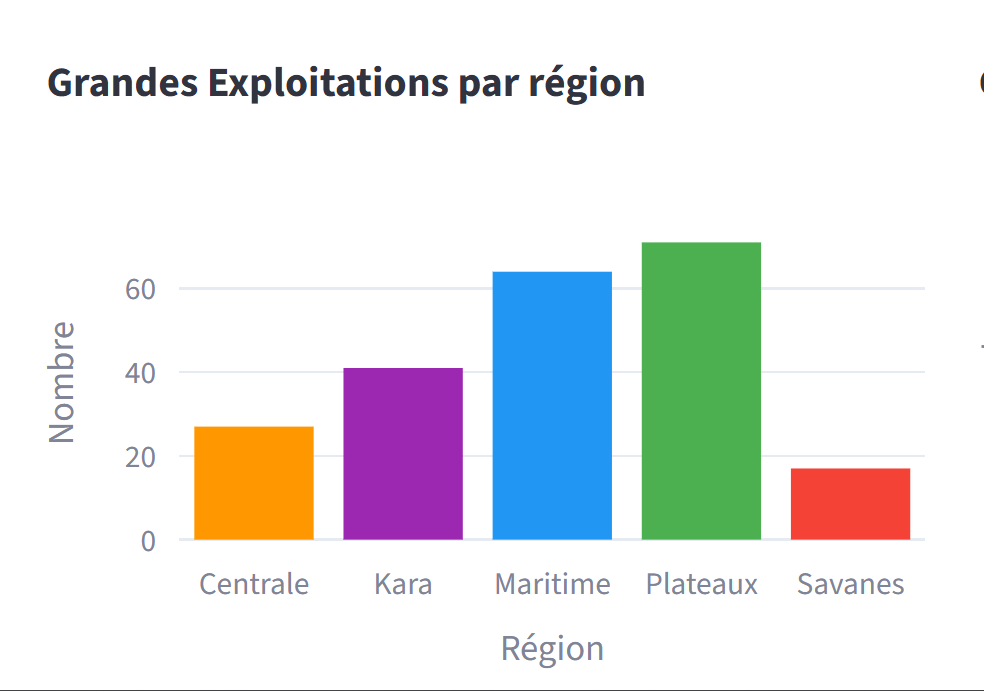
\includegraphics[width=\textwidth]{figures/fig3a.png}
        \caption{Grandes exploitations par région}
        \label{fig:grandes_region}
    \end{subfigure}
    \hfill
    \begin{subfigure}[b]{0.48\textwidth}
        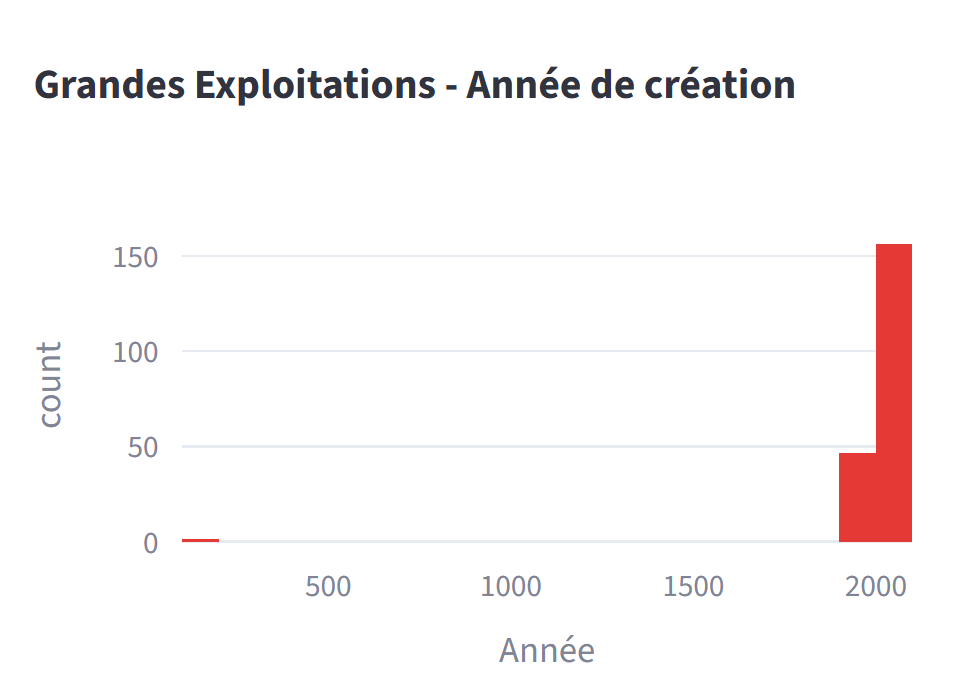
\includegraphics[width=\textwidth]{figures/Fig3b.png}
        \caption{Année de création des grandes exploitations}
        \label{fig:annee_creation}
    \end{subfigure}
    \caption{Analyse des grandes exploitations agricoles}
    \label{fig:grandes_exploit}
\end{figure}

Avec \textbf{220 grandes exploitations} recensées, ce segment reste minoritaire mais stratégique.
L'analyse temporelle de l'année de création révèle une dynamique de création d'exploitations
s'accélérant à partir des années 2000, avec un pic notable dans les années 2010--2020, période
marquée par diverses politiques d'investissement agricole.

\subsection{Top 15 des préfectures - Petites exploitations}

\begin{figure}[H]
    \centering
    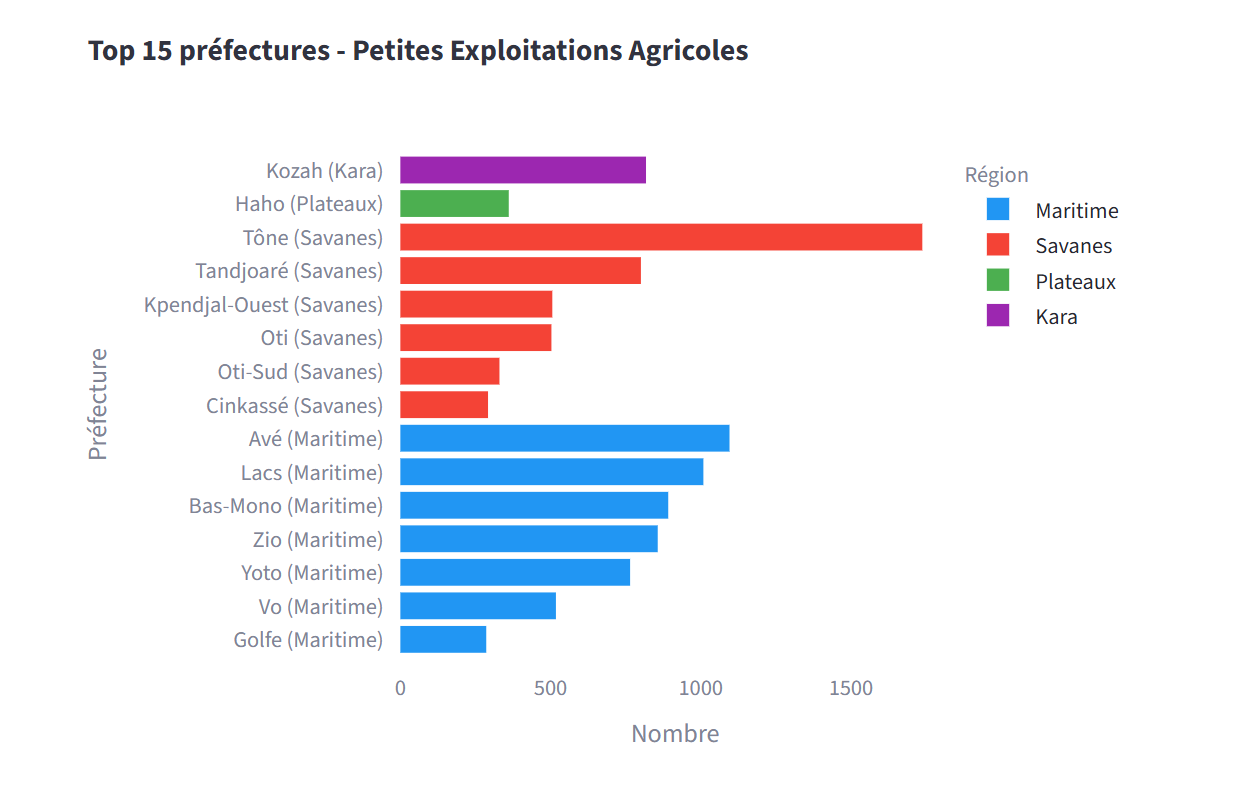
\includegraphics[width=\textwidth]{figures/fig4.png}
    \caption{Top 15 préfectures par nombre de petites exploitations agricoles}
    \label{fig:top15}
\end{figure}

L'analyse à l'échelle des préfectures permet d'identifier les bassins agricoles les plus denses. Les
préfectures des régions Maritime et Plateaux dominent ce classement, confirmant la vocation
agricole historique de ces territoires.

% ============================================================
\section{Réseau coopératif agricole}
% ============================================================

\subsection{Ampleur et structure du réseau}

Avec \textbf{6 859 coopératives agricoles} recensées sur l'ensemble du territoire, le Togo dispose
d'un réseau associatif agricole relativement développé. Ce maillage coopératif joue un rôle essentiel
dans l'accès aux intrants, la mutualisation des équipements et la commercialisation des productions.

\begin{figure}[H]
    \centering
    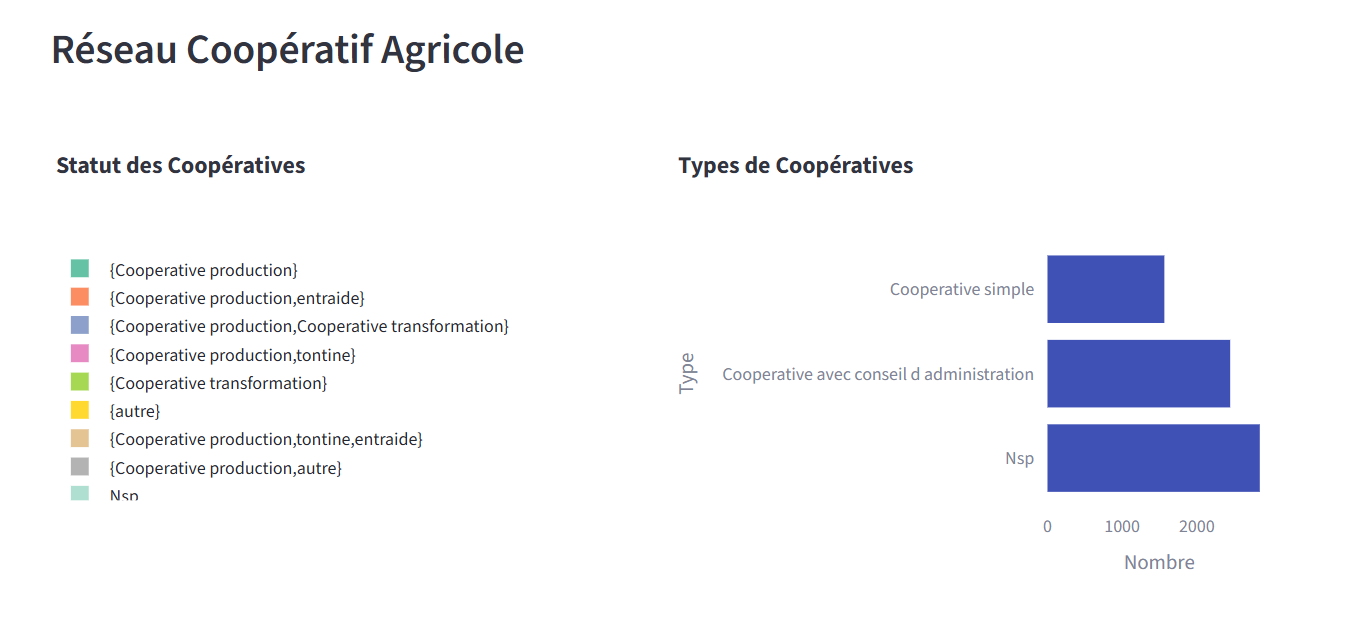
\includegraphics[width=\textwidth]{figures/fig5.png}
    \caption{Analyse du réseau coopératif - Statuts et types}
    \label{fig:cooperatif}
\end{figure}

\subsection{Typologies des coopératives}

L'analyse des statuts et types de coopératives met en évidence trois catégories principales :

\begin{itemize}[leftmargin=1.5em]
    \item \textbf{Coopératives simples} : forme la plus répandue, structurées autour d'une activité
          productive commune (cultures vivrières, maraîchage) ;
    \item \textbf{Coopératives avec conseil d'administration} : structures plus formalisées, souvent
          bénéficiaires d'appuis institutionnels ;
    \item \textbf{Non spécifiés (NSP)} : coopératives dont le statut n'a pas été renseigné lors du
          recensement, représentant un angle mort des données.
\end{itemize}

Les types de coopératives les plus fréquents incluent les coopératives de \textit{production},
de \textit{transformation} et les coopératives de type \textit{ESOP} (Entreprise de Services et
Organisations de Producteurs), ces dernières étant particulièrement développées dans certaines
filières comme le riz et le soja.

\subsection{Distribution géographique des coopératives}

\begin{figure}[H]
    \centering
    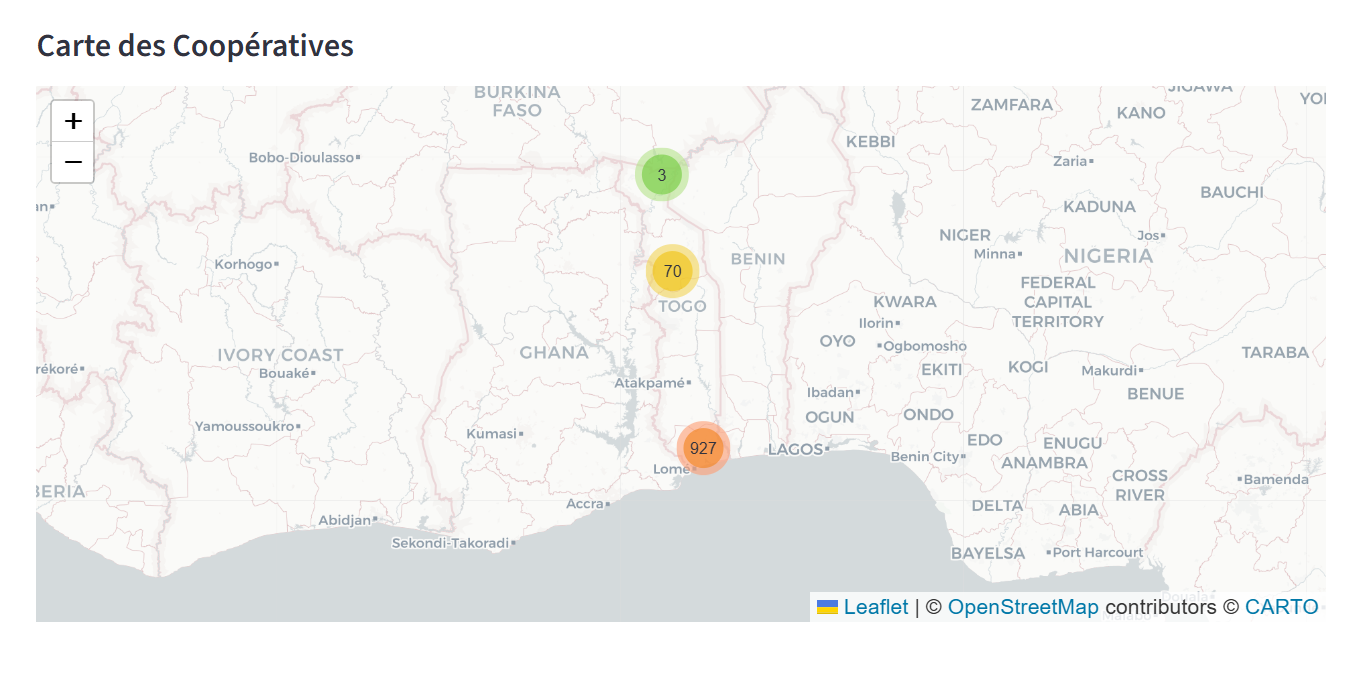
\includegraphics[width=\textwidth]{figures/fig6.png}
    \caption{Carte de distribution des coopératives agricoles}
    \label{fig:carte_coop}
\end{figure}

La concentration des coopératives suit globalement la même logique que celle des petites exploitations,
avec une prédominance dans les régions Maritime et Plateaux. Toutefois, certaines préfectures des
régions Kara et Centrale présentent une densité coopérative notable, témoignant de programmes
d'appui spécifiques à ces territoires.

% ============================================================
\section{Couverture des Zones d'Aménagement Agricole Planifiées (ZAAPs)}
% ============================================================

\subsection{Présentation des ZAAPs}

Les Zones d'Aménagement Agricole Planifiées (ZAAPs) et les Zones d'Aménagement de Petits Bassins
(ZAPBs) constituent des infrastructures stratégiques du développement agricole togolais. Ces
périmètres aménagés visent à moderniser la production agricole en offrant des conditions optimales
(irrigation, organisation parcellaire, accès aux intrants) à des groupes de producteurs organisés.

\subsection{État des lieux}

\begin{table}[H]
\centering
\caption{Indicateurs clés des ZAAPs et ZAPBs}
\label{tab:zaaps}
\renewcommand{\arraystretch}{1.3}
\begin{tabular}{lr}
\toprule
\textbf{Indicateur} & \textbf{Valeur} \\
\midrule
Nombre de périmètres (formes surfaciques) & 144 \\
Nombre de champs individuels & 1 883 \\
Nombre de préfectures couvertes & 28+ \\
Ratio champs/périmètre (moyen) & $\approx$ 13 \\
\bottomrule
\end{tabular}
\end{table}

\begin{figure}[H]
    \centering
    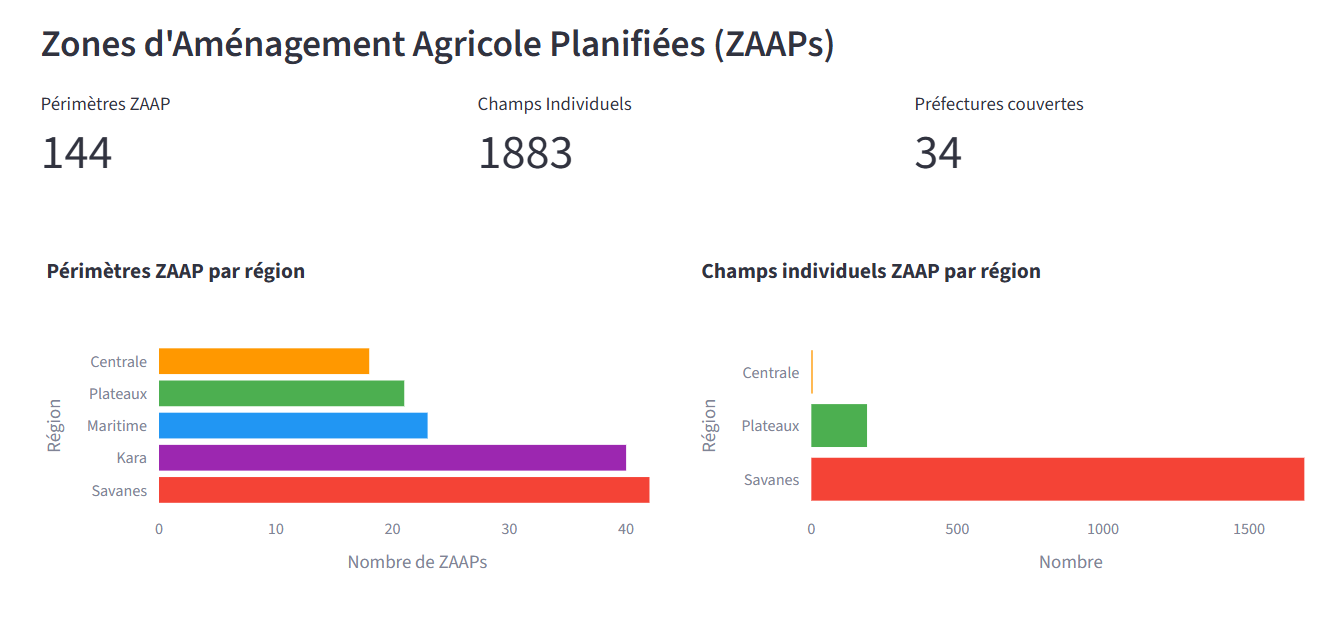
\includegraphics[width=\textwidth]{figures/fig7.png}
    \caption{Distribution des ZAAPs par région et types d'organisation}
    \label{fig:zaaps_analyse}
\end{figure}

\subsection{Répartition géographique}

L'analyse de la distribution des périmètres ZAAPs par région révèle une concentration dans les régions
des \textbf{Plateaux} et \textbf{Savanes}, ce qui reflète les priorités d'aménagement hydro-agricole
dans des zones à fort potentiel mais insuffisamment valorisées. La région Maritime, bien qu'agricole,
bénéficie moins de ce type d'infrastructure du fait de son accès plus facile à l'eau et de la prédominance
d'exploitations privées.

\begin{figure}[H]
    \centering
    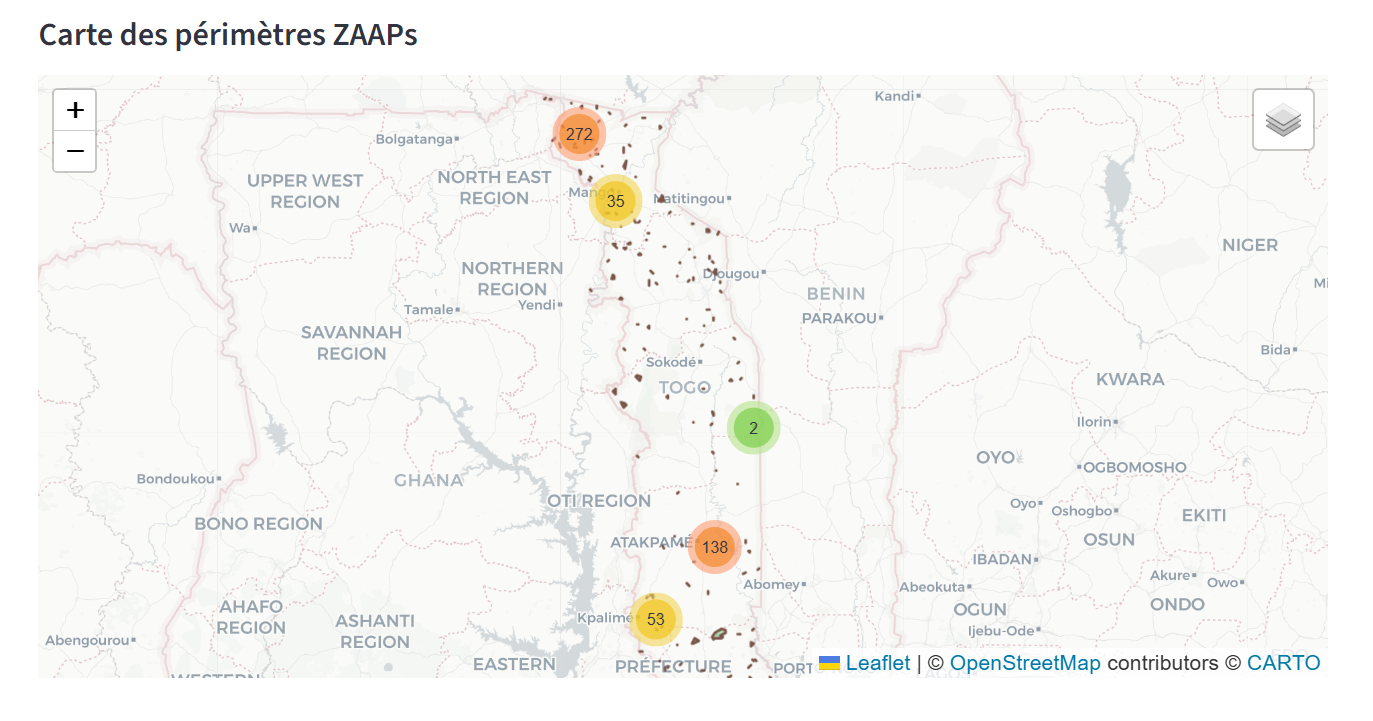
\includegraphics[width=\textwidth]{figures/fig8.png}
    \caption{Carte des périmètres ZAAPs et champs individuels}
    \label{fig:carte_zaaps}
\end{figure}

\subsection{Types d'organisation dans les champs ZAAP}

L'analyse des types d'organisation au sein des champs individuels révèle une diversité de formes
collectives : coopératives de production, tontines, groupes d'entraide, et champs collectifs de ZAAP.
Cette pluralité des modes d'organisation témoigne de la richesse des pratiques communautaires
agricoles au Togo.

% ============================================================
\section{Marchés et accessibilité aux services agricoles}
% ============================================================

\subsection{Le réseau des marchés}

Les marchés agricoles constituent des nœuds essentiels du système agro-alimentaire togolais,
assurant la connexion entre producteurs et consommateurs. L'analyse recense \textbf{1 078 marchés}
répartis sur l'ensemble du territoire.

\begin{figure}[H]
    \centering
    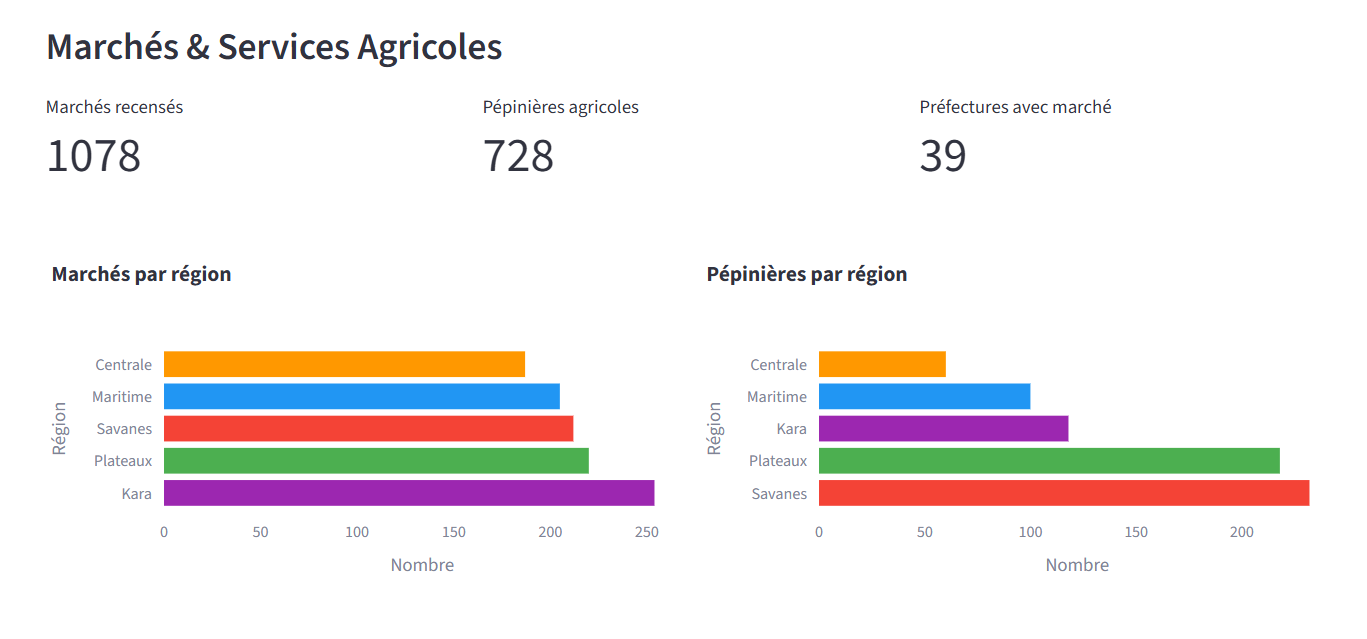
\includegraphics[width=\textwidth]{figures/fig9.png}
    \caption{Analyse des marchés et services agricoles}
    \label{fig:marches}
\end{figure}

\subsection{Fréquence d'ouverture}

L'analyse des jours d'ouverture des marchés révèle plusieurs régimes de fonctionnement :

\begin{itemize}[leftmargin=1.5em]
    \item \textbf{Marchés quotidiens (7j/7)} : principalement localisés dans les zones urbaines et
          périurbaines, notamment autour de Lomé et des grandes villes ;
    \item \textbf{Marchés hebdomadaires (1 à 3 jours/semaine)} : dominant dans les zones rurales,
          correspondant aux marchés périodiques traditionnels qui rythment la vie économique locale ;
    \item \textbf{Marchés semi-permanents (4 à 6 jours/semaine)} : forme intermédiaire, souvent
          observée dans les chefs-lieux de préfecture.
\end{itemize}

\subsection{Les pépinières agricoles}

Les \textbf{728 pépinières agricoles} recensées constituent un maillon crucial de la chaîne de valeur
agricole, assurant l'approvisionnement en plants et semences. Leur répartition géographique indique
une concentration dans les régions Maritime et Plateaux, en corrélation avec la densité d'exploitations
agricoles dans ces zones.

\begin{figure}[H]
    \centering
    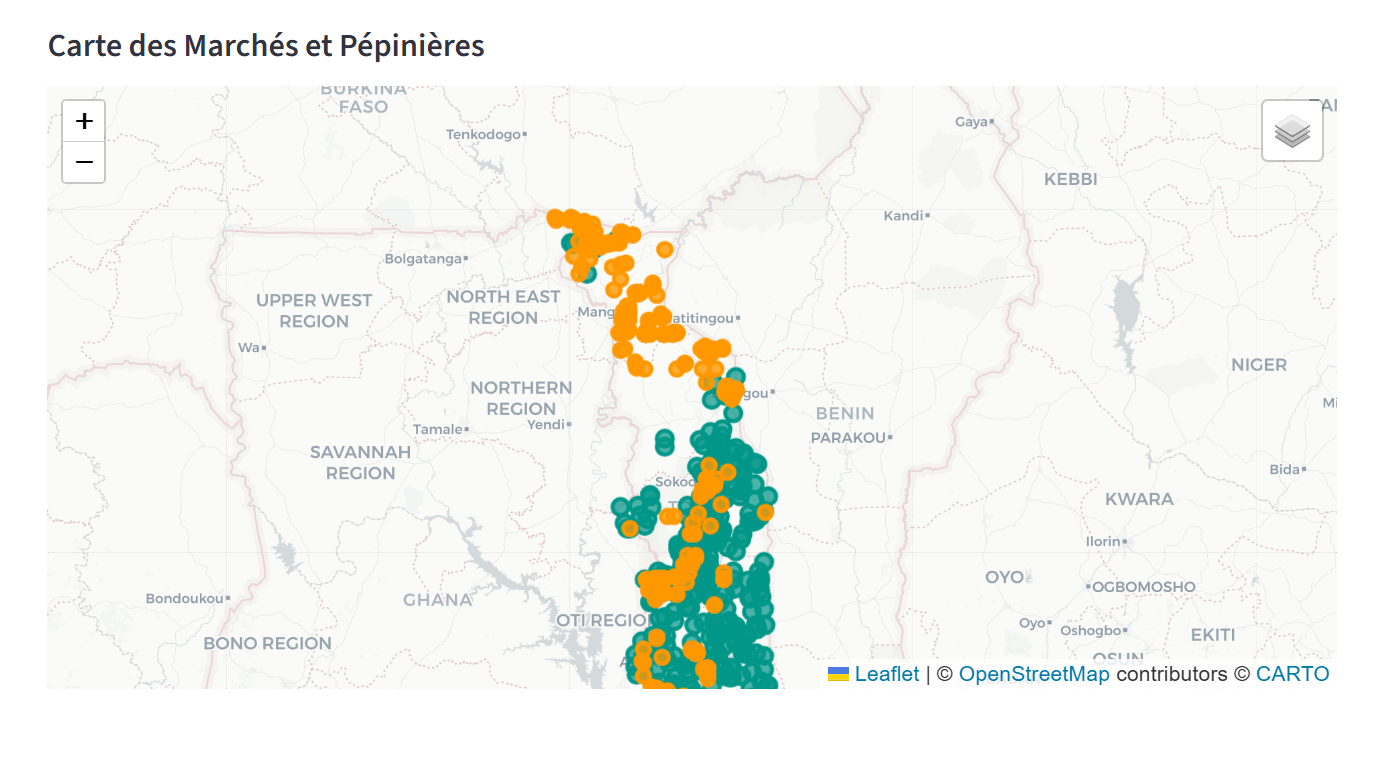
\includegraphics[width=\textwidth]{figures/fig10.png}
    \caption{Carte des marchés et pépinières agricoles}
    \label{fig:carte_marches}
\end{figure}

L'analyse du type de terrain des pépinières révèle une prédominance du \textit{privé individuel},
confirmant que l'offre en plants repose essentiellement sur des opérateurs privés, avec une
contribution plus limitée du secteur public et des groupements.

% ============================================================
\section{Synthèse et recommandations}
% ============================================================

\subsection{Principaux enseignements}

Cette analyse géospatiale du tissu agricole togolais permet de dégager plusieurs enseignements majeurs :

\begin{enumerate}[leftmargin=1.5em]
    \item \textbf{Forte concentration méridionale} : les régions Maritime et Plateaux concentrent
          la majorité des entités agricoles, reflétant des avantages comparatifs historiques (climat,
          sols, densité de population). Cette concentration crée un risque de sous-valorisation des
          potentiels agricoles des régions Nord.

    \item \textbf{Prédominance de l'agriculture familiale} : avec plus de 13 000 petites exploitations
          recensées, l'agriculture togolaise reste essentiellement familiale et de subsistance. Les
          politiques de modernisation doivent s'adapter à cette réalité.

    \item \textbf{Un réseau coopératif dense mais inégalement réparti} : les 6 859 coopératives
          constituent un atout majeur pour la structuration des filières, mais leur concentration dans
          certaines zones laisse d'autres territoires insuffisamment structurés.

    \item \textbf{Des ZAAPs insuffisamment déployées} : avec seulement 144 périmètres aménagés
          pour l'ensemble du territoire, la couverture en infrastructures d'aménagement hydroagricole
          reste limitée au regard du potentiel irrigable identifié.

    \item \textbf{Un accès aux marchés globalement assuré} : le réseau de 1 078 marchés offre
          une couverture territoriale satisfaisante, bien que certaines zones rurales enclavées
          restent sous-desservies.
\end{enumerate}

\subsection{Recommandations}

Sur la base de ces analyses, plusieurs recommandations peuvent être formulées :

\begin{itemize}[leftmargin=1.5em]
    \item \textbf{Intensifier les investissements dans les ZAAPs des régions Nord} (Kara, Savanes)
          pour réduire les disparités territoriales et valoriser le potentiel irrigable de ces zones ;

    \item \textbf{Renforcer la structuration coopérative} dans les préfectures à faible densité
          coopérative, notamment dans les régions Centrale et Kara ;

    \item \textbf{Appuyer la mise à niveau des grandes exploitations} (220 recensées) en les dotant
          d'accès privilégiés aux services (conseil agricole, crédit, marchés de gros) ;

    \item \textbf{Développer le réseau de pépinières} dans les régions déficitaires pour garantir
          un approvisionnement en plants de qualité sur l'ensemble du territoire ;

    \item \textbf{Combler les lacunes des données} : un effort de mise à jour et de complétude
          des données (champs ``NSP'') est nécessaire pour améliorer la qualité des analyses futures.
\end{itemize}

% ============================================================
\section{Conclusion}
% ============================================================

Ce rapport présente les résultats d'une analyse géospatiale approfondie du tissu agricole togolais,
réalisée dans le cadre du Data Challenge Agriculture \#1 du Togo AI Lab. En exploitant
\textbf{26 942 enregistrements} issus de huit jeux de données géospatiales libres, le tableau de
bord interactif développé offre une vision exhaustive et granulaire de la géographie agricole
du Togo.

Les analyses menées mettent en lumière la richesse et la diversité du secteur agricole togolais,
tout en révélant des disparités territoriales importantes entre le Nord et le Sud du pays. Les
outils de visualisation interactifs développés, cartes par clusters, graphiques statistiques,
filtres régionaux  constituent un support de décision concret pour les décideurs, les
organisations de développement et les acteurs du secteur privé agricole.

La démocratisation des données géospatiales ouvertes, combinée aux capacités modernes de
visualisation et d'analyse, ouvre des perspectives inédites pour le pilotage des politiques
agricoles au Togo. Ce travail s'inscrit pleinement dans cette dynamique, en démontrant
la valeur ajoutée que l'analyse de données peut apporter au service du développement agricole.

\vspace{1.5cm}

\begin{center}
\textit{``Une donnée. Une idée. Un impact.''}\\[0.3em]
\small -- Togo AI Lab, Data Challenge Agriculture \#1
\end{center}

% ============================================================
\appendix
\section{Annexe - Description des variables clés}
% ============================================================

\begin{longtable}{p{4cm} p{4cm} p{6.5cm}}
\toprule
\textbf{Variable} & \textbf{Dataset(s)} & \textbf{Description} \\
\midrule
\endhead
\texttt{region\_nom\_bdd} & Tous & Nom de la région administrative \\
\texttt{prefecture\_nom\_bdd} & Tous & Nom de la préfecture \\
\texttt{commune\_nom\_bdd} & Tous & Nom de la commune \\
\texttt{canton\_nom\_bdd} & Tous & Nom du canton \\
\texttt{nom\_localite} & Tous & Nom de la localité \\
\texttt{geometry} & Tous & Géométrie WKT (POINT, POLYGON, MULTIPOLYGON) \\
\texttt{exploitation\_nom} & Grandes, Plantations & Nom de l'exploitation ou de la plantation \\
\texttt{exploitation\_annee} & Grandes, Plantations & Année de création de l'exploitation \\
\texttt{terrain} & Plantations, Pépinières & Type de tenure foncière \\
\texttt{cooperative\_nom} & Coopératives, Petites, ZAAPs & Nom de la coopérative \\
\texttt{cooperative\_type} & Coopératives, Petites, ZAAPs & Type d'organisation coopérative \\
\texttt{cooperative\_statut} & Coopératives & Statut juridique de la coopérative \\
\texttt{marche\_nom} & Marchés & Nom du marché \\
\texttt{jour} & Marchés & Jours d'ouverture du marché \\
\texttt{organisme} & Marchés & Organisme gestionnaire \\
\texttt{zaap\_nom} & ZAAPs formes & Nom du périmètre ZAAP \\
\texttt{etab\_nom} & Pépinières & Nom de l'établissement \\
\texttt{etab\_creation\_date} & Pépinières & Année de création de la pépinière \\
\bottomrule
\end{longtable}

\section{Annexe - Architecture du tableau de bord}

Le tableau de bord interactif est structuré en \textbf{5 onglets thématiques} :

\begin{enumerate}[leftmargin=1.5em]
    \item \textbf{Carte Interactive} : visualisation géospatiale multi-couches avec clustering,
          contrôle des couches et légende ;
    \item \textbf{Densités \& Distributions} : graphiques en barres empilées, treemap global,
          histogrammes temporels et classement des préfectures ;
    \item \textbf{Réseau Coopératif} : analyse des statuts et types, distribution géographique
          et carte dédiée aux coopératives ;
    \item \textbf{Couverture ZAAPs} : analyse des périmètres et champs individuels, types
          d'organisation et carte des aménagements ;
    \item \textbf{Marchés \& Services} : analyse des marchés (fréquence, localisation) et
          des pépinières (type de terrain, répartition).
\end{enumerate}

Un filtre régional en sidebar permet de restreindre l'ensemble des analyses à une région spécifique,
offrant une vision territoriale fine aux décideurs locaux.

\end{document}
